% --------------------------------------------------------------
% Abhi's Standard math Preamble.
% --------------------------------------------------------------
 
% Document packages / layout
\documentclass[pdf,12pt]{beamer}
\usetheme{Copenhagen}
\usecolortheme{seahorse}

% Figure Packages
\usepackage{float}
\usepackage{hyperref}
\usepackage{subcaption}
\usepackage{wrapfig}
\usepackage[export]{adjustbox} %center option in include graphics

% Math Packages
\usepackage{amsmath,amsthm,amssymb,mathrsfs,bm}
\usepackage{mathtools}
\usepackage{commath}
\usepackage{esvect} %For derivatives of vectors \vec{u}' -> \vv{u}'

% Code input 
\usepackage{algorithm}
\usepackage{algpseudocode}

% Quality of Life Packages
\usepackage{enumerate}

\newcommand{\course}{\mathcal{G}}
\newcommand{\fine}{\mathcal{F}}

\newtheorem*{lemma*}{Lemma}
\newtheorem*{theorem*}{Theorem}
 
\title{An Investigation into Parareal}
\author{Abhijit Chowdhary} 
\institute{New York University}
\date{May 2019}

\begin{document}
 
\frame{\titlepage}

\begin{frame}
  \frametitle{Problem Statement}
  We would like to numerically solve the autonomous ordinary differential
  equation:
  \begin{equation*}
    \begin{cases}
      u'(t) = f(t, u), & t \in [t_0, t_f] \\
      u(t_0) = u_0
    \end{cases}
  \end{equation*}
  where $f : \mathbb{R}^d \to \mathbb{R}^d$ and $u: \mathbb{R} \to \mathbb{R}^d$.

  Framing this in a HPC context, how can we solve the above while taking
  advantage of massively parallel hardware?
\end{frame}

\begin{frame}
  \frametitle{Serial Methods}
  \begin{itemize}
    \item <1-> Forward and Backward Euler:
      \[
        u_{n+1} = u_n +  h f(t, u_n), u_n + h f(t,u_{n+1})
      \]
    \item <2-> Linear Multistep Methods
      \[
        \sum_k \alpha_k y_{n+k} = h\sum_k\beta_k f(t_{n+k},y_{n+k})
      \]
    \item <3-> Runge Kutta Methods
    \item <4-> Etc.
  \end{itemize}
\end{frame}

\begin{frame}
  \frametitle{Parallel Techniques}
  \begin{alertblock}{Problem!}
    Most of the previous methods are iterative, depending on the previously
    computed values.
  \end{alertblock}
  Not embarrassingly parallel... We have to get creative.
\end{frame}

\begin{frame}
  \frametitle{Parallel-In-Time}
  One technique is to parallelize the problem across time, i.e. split $[t_0,
  t_f]$ into slices $[t_n, t_{n+1}]$ and in parallel solve each slice.
  \begin{block}{Iteration Dependence}
    But since each slice depends on the previous, how can we chain together
    these individual solutions to each slice?
  \end{block}
\end{frame}

\begin{frame}
  \frametitle{Parareal}
  \begin{alertblock}{Predictor-Corrector}
    What if we were to predict the portions that $[t_n, t_{n+1}]$ are dependent
    on with a cheap course operator, and then correct with a fine operator!
  \end{alertblock}
  Yes!
\end{frame}

\begin{frame}
  \frametitle{Parareal}
  Let $\mathcal{G}$ be a course and inexpensive operator, and let $\mathcal{F}$
  be a fine operator of high order. Then Parareal iteration is:
  \[
    \lambda_{n+1}^{k+1} = \mathcal{G}(t_{n+1},t_n,\lambda_n^{k+1}) + 
    \mathcal{F}(t_{n+1},t_n,\lambda_n^k) - \mathcal{G}(t_{n+1},t_n,\lambda_n^k)
  \]
  \begin{block}{Parallel Potential}
    Notice! The $\mathcal{F}$ term depends only on the previous solutions, which
    means it can be computed in parallel for each $k$ step. Furthermore,
    $\mathcal{G}(\lambda_n^k)$ satisfies the FSAL property!
  \end{block}
\end{frame}

\begin{frame}
  \frametitle{Parareal: Visual Example}
  \begin{center}
    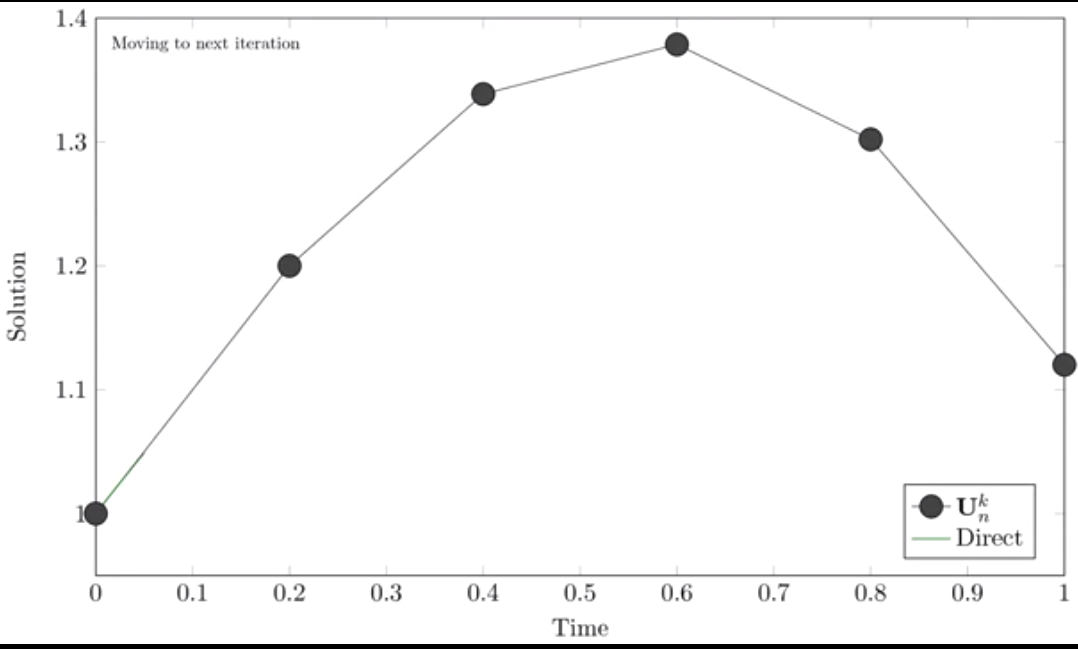
\includegraphics[width=.9\textwidth]{./resources/Parareal1}
  \end{center}
  Full beautiful animation found on wikipedia's Parareal page.
\end{frame}
\begin{frame}
  \frametitle{Parareal: Visual Example}
  \begin{center}
    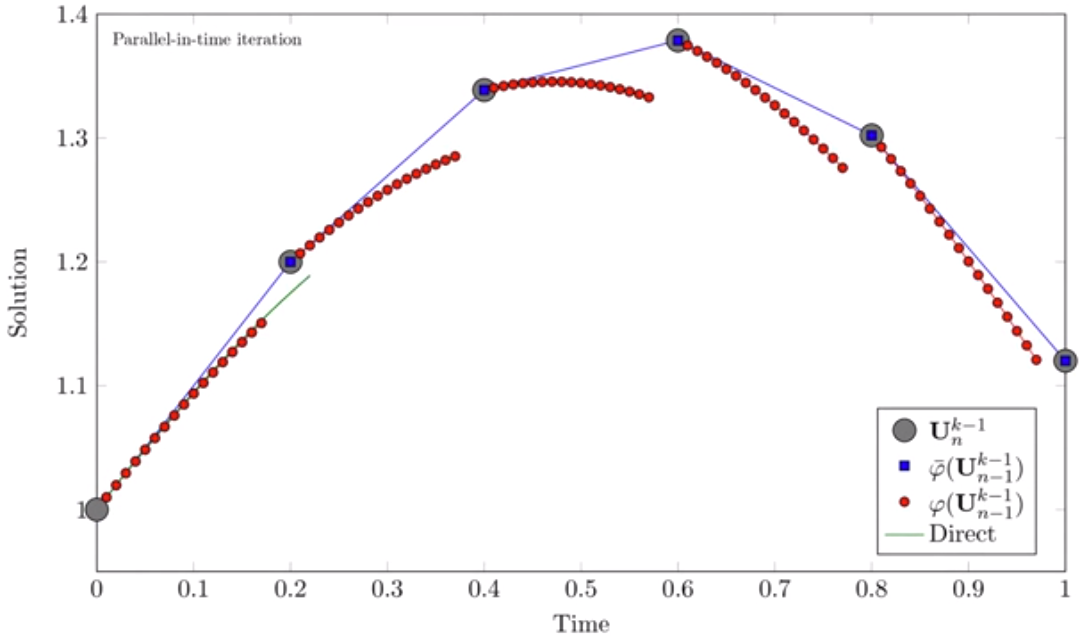
\includegraphics[width=.9\textwidth]{./resources/Parareal2}
  \end{center}
  Full beautiful animation found on wikipedia's Parareal page.
\end{frame}
\begin{frame}
  \frametitle{Parareal: Visual Example}
  \begin{center}
    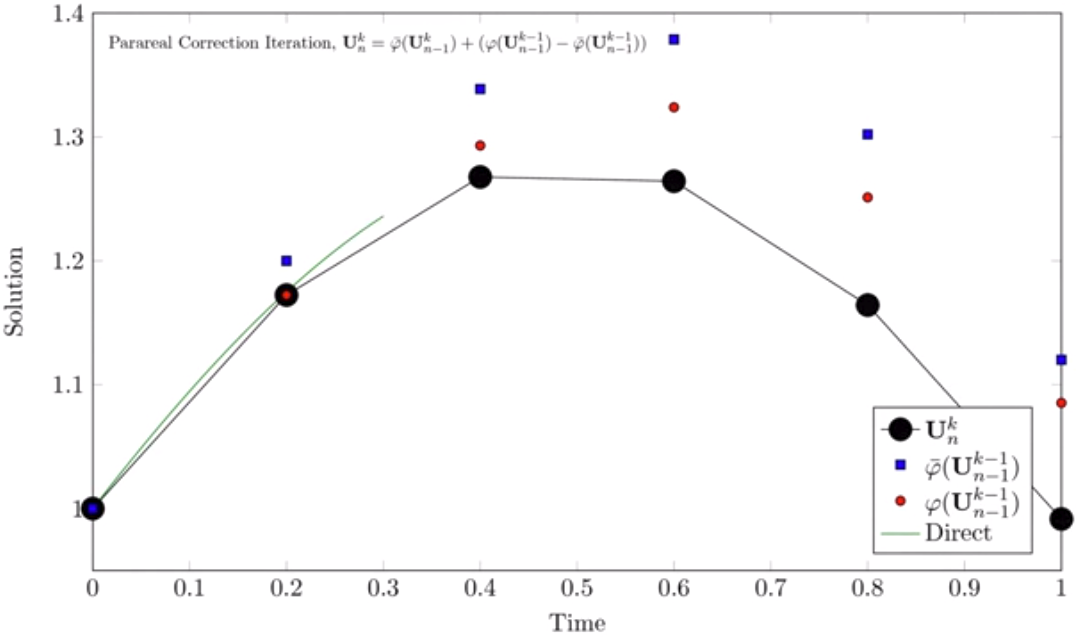
\includegraphics[width=.9\textwidth]{./resources/Parareal3}
  \end{center}
  Full beautiful animation found on wikipedia's Parareal page.
\end{frame}

\begin{frame}
  \frametitle{Pseudocode}
  \begin{algorithmic}
    \Require $y_0$ and course and fine solvers $\course$, $\fine$.
    \State $y_c \gets \course(t_f, t_0, y_0)$.\Comment{Coarsely approximate
      solution}
    \State $y \gets y_c$.
    \While{$\textrm{iter} < \textrm{max\_iter}\ \&\&$ not converged}
      \For{$n = 0 \to P$}\Comment{Parallel capable}
        \State $y_f(n) = \fine(t_{n+1},t_n,y(n))$.
        \State $\delta y(n) = y_f(n) - y_c(n)$.\Comment{corrector term. FSAL}
      \EndFor
      \For{$n = 0 \to P$}
        \State $y_c(n) = \course(t_{n+1},t_n,y(n))$.\Comment{Predict.}
        \State $y(n) = y_c(n) + \delta y(n)$.\Comment{Correct.}
      \EndFor
    \EndWhile
  \end{algorithmic}
\end{frame}

\begin{frame}
  \frametitle{Parallel Pseudocode}
  \begin{algorithmic}
    \Require $y_0$ and course and fine solvers $\course$, $\fine$.
    \State $y_c \gets \course(t_f, t_0, y_0)$.\Comment{Coarsely approximate
      solution}
    \State $y \gets y_c$.
    \While{$\textrm{iter} < \textrm{max\_iter}\ \&\&$ not converged}
      \State \#pragma omp parallel for
      \For{$n = 0 \to P$}
        \State $y_f(n) = \fine(t_{n+1},t_n,y(n))$.
        \State $\delta y(n) = y_f(n) - y_c(n)$.\Comment{corrector term. FSAL}
      \EndFor
      \For{$n = 0 \to P$}
        \State $y_c(n) = \course(t_{n+1},t_n,y(n))$.\Comment{Predict.}
        \State $y(n) = y_c(n) + \delta y(n)$.\Comment{Correct.}
      \EndFor
    \EndWhile
  \end{algorithmic}
\end{frame}

\begin{frame}
  \frametitle{Speedup Analysis}
  Suppose we have $P$ processors, and suppose our fine method takes $T_f$ time,
  $T_g$ for the course method. Furthermore, assume that our Parareal iteration
  needs $k$ steps. Then the speedup it provides is:
  \[
    S = \frac{PT_f}{PT_g + k(PT_g + T_f)} 
    = \frac{1}{\frac{T_g}{T_f} + k(\frac{T_g}{T_f} + \frac{1}{P})} 
    = \frac{1}{\frac{T_g}{T_f}(1+k) + \frac{k}{P}} 
  \]
  Note:
  \[
    \lim_{P \to \infty} \frac{1}{\frac{T_g}{T_f}(1+k) + \frac{k}{P}} =
    \frac{T_f}{T_g(1+k)}
  \]
\end{frame}
\begin{frame}
  \frametitle{No Free Lunch}
  \[
    S_\infty = \frac{T_f}{T_g(1+k)}
  \]
  This tells us something very important, we want the ratio $T_f / T_g$ to be as
  large as possible, and we want $k$ to be as small as possible.
  \begin{block}{Theorem}
    The parareal method has order of accuracy $mk$, where $k-1$ is the number of
    parareal iterations made and $m$ is the order of $\course$, assuming $\fine$
    is close to truth. (Bal) 
  \end{block}
  Therefore, we have this uncomfortable optimization problem. We want $k$ small
  for speedup, but large for order. If we make $m$ large instead, then the ratio
  $T_f/T_g$ becomes smaller...
\end{frame}

\begin{frame}
  \frametitle{Strong Scaling}
  \begin{center}
    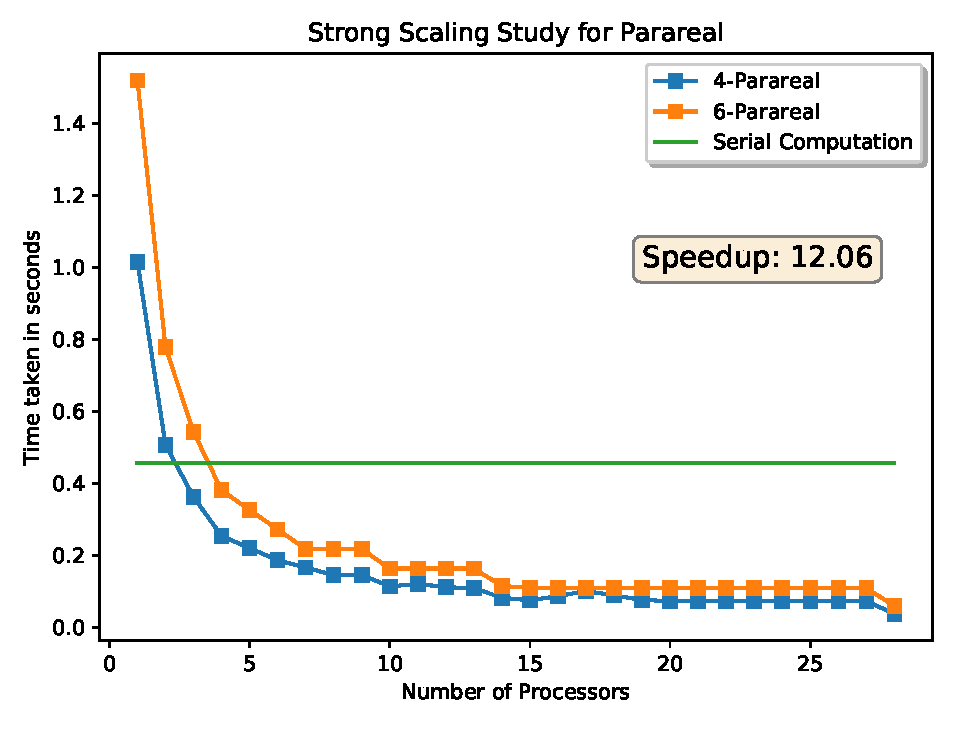
\includegraphics[width=.8\textwidth]{./resources/strong_scaling}
  \end{center}
\end{frame}

\begin{frame}
  \frametitle{Weak Scaling}
  \begin{center}
    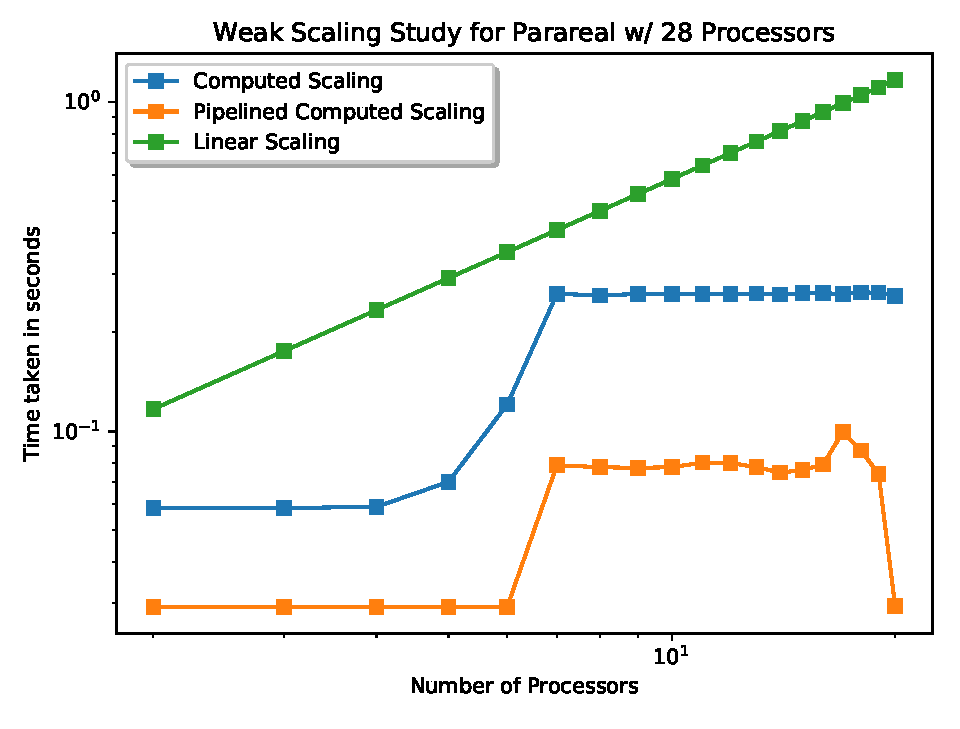
\includegraphics[width=.8\textwidth]{./resources/weak_scaling}
  \end{center}
\end{frame}

\begin{frame}
  \frametitle{Improvements $\mid$ Pipelined Parareal}
  \begin{center}
    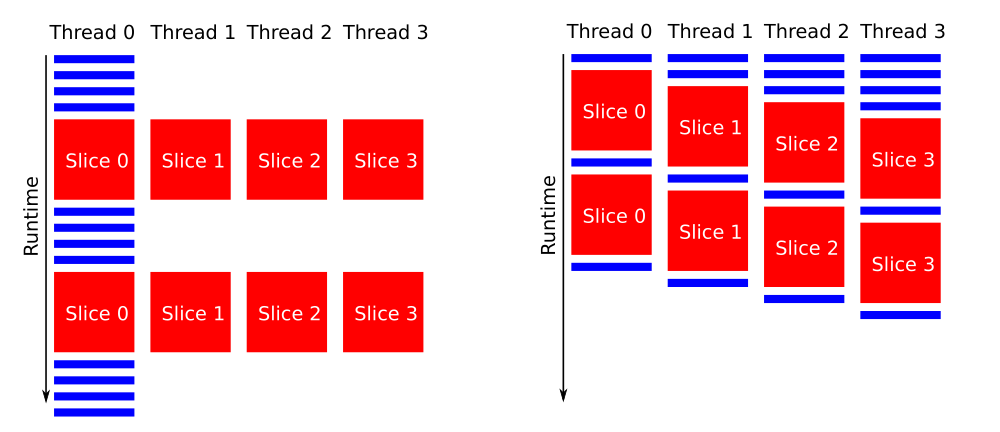
\includegraphics[width=\textwidth]{./resources/pipelined_parareal}
  \end{center}
  Figure borrowed from Ruprecht's \textit{Implementing Parareal}.
\end{frame}

\begin{frame}
  \frametitle{Pipelined Parareal Pseudocode}
  It's a bit too complicated to present in a slide, but the general idea is to
  begin the omp parallel statement at the beginning and then pretend like were
  in a MPI enviornment.
  \begin{block}{General Idea}
    Thread $p$ processes the new iteration at $p+1$. MPI communication is
    mimicked with locks, and done in place.
  \end{block}
\end{frame}


\end{document}
